\documentclass{beamer}

\usepackage{bera}
\usepackage{hyperref}
\usepackage{genom}
\usepackage{listings}
\usepackage{tabularx}
\usepackage{amssymb}

\usetheme{Rochester}

\graphicspath{{./figures/}}

\newcommand{\figw}[2]{
        \centerline{ \includegraphics[width=#2]{#1}}}
\newcommand{\figc}[3]{
        \centerline{
          \parbox{#2}{\includegraphics[width=#2]{#1}\\
        \centerline{
	  {\em\footnotesize #3}}}}}

\newcommand{\bi}{\begin{itemize}\itemsep 0mm}
\newcommand{\ei}{\end{itemize}}
\newcommand{\be}{\begin{enumerate}\itemsep 0mm}
\newcommand{\ee}{\end{enumerate}}
\newcommand{\bd}{\begin{description}\itemsep 0mm}
\newcommand{\ed}{\end{description}}

\lstset{frame=single}
%-------------------------------------------------
\title{The Generator of Modules \\ \GenoM{}}
 
\author{Sara Fleury - Matthieu Herrb}
 
\institute{
\includegraphics[height=2cm]{openlogo}}
\date{November 2010}


\AtBeginSection[]{
\begin{frame}<beamer>
\frametitle{Agenda}
\tableofcontents[currentsection]
\end{frame}
}
%-------------------------------------------------


\begin{document}

\begin{frame}[plain]
\titlepage
\end{frame}

\begin{frame}
  \frametitle{Agenda}
  \tableofcontents
\end{frame}


%----------------------------------------------------------------------
\section{General presentation}
\label{gene}
%----------------------------------------------------------------------
\begin{frame}
\frametitle{\GenoM{}: Generator of Modules}

\begin{center}
\begin{tabularx}{\linewidth}{p{3cm}Xp{3cm}}
 \figc{adam-detour-web-small.jpg}{1.75cm}{adam} &
 \figc{junior-detour-web-small.jpg}{1.25cm}{junior} &
 \figc{lama-detour-web-small.jpg}{1.75cm}{lama} \\

 \figc{h2-detour-web-small.jpg}{2cm}{h2} &
 \figc{h2bis-detour-web-small.jpg}{1.6cm}{h2bis} &
 \figc{lapa-detour-web-small.jpg}{1.5cm}{lapa} \\

 \figc{karma-detour-web-small.jpg}{3cm}{karma} &
 \figc{diligent-detour-web-small.jpg}{0.8cm}{diligent} &
 \figc{scouts-detour-web-small.jpg}{1.2cm}{scout} \\
\end{tabularx}
\end{center}
\end{frame}

%----------------------------------------------------------------------
\begin{frame}
\frametitle{\GenoM{}: Generator of Modules}

\begin{center}
\begin{tabularx}{\linewidth}{p{3cm}Xp{3cm}}
 \figc{dala-detour-web-small.jpg}{1.6cm}{dala} &
 \figc{rackham-detour-web-small.jpg}{0.7cm}{rackham} &
 \figc{jidowanki-detour-web-small.jpg}{1.6cm}{jido} \\
\figc{lhassa-detour-web-small.jpg}{2cm}{lhassa}
& \figc{hrp2.pdf}{1cm}{hrp2} & \figc{PatrolDX.jpg}{1cm}{Pioneer / Player} 
\end{tabularx}
\end{center}
\end{frame}

%----------------------------------------------------------------------
\begin{frame}
\frametitle{\GenoM{}: Generator of Modules}

Tool to integrate processing functions into independant servers or \textbf{modules}

\figw{./figures/module-simple}{5.5cm}

\textbf{Activity:} function in processing

\textbf{Reports:} ``incorrect-parameters'', ``solution-not-found'', 
``not-enough-memory'', ``unforeseen-case''

\end{frame}

%----------------------------------------------------------------------
\begin{frame}
\frametitle{Why encapsulate functions ?}

\centerline{ \textbf{Software integration on embedded systems} }

\vspace{1em}
 \textbf{Requirements:} 

	\begin{itemize}

	\item Controllable system
		\begin{itemize}

		\item processing start/stop
		\item dynamic parametrization
		\item error recovery
		\end{itemize}

	\item Communicating system
		\begin{itemize}
		\item data transfers
		\item use of other functions
		\end{itemize}
	\end{itemize}


\end{frame}

%----------------------------------------------------------------------
\begin{frame}
\frametitle{Why encapsulate functions (cont.)}

 \textbf{Requirements (cont.) } 


	\begin{itemize}
	\item Standard interfaces
		\begin{itemize}
		\item list of available functions
		\item Data structures of input/outputs
		\item Validity domains
		\item List of failure reports
		\end{itemize}

	\item Standard organization of files

	\end{itemize}

\end{frame}

%----------------------------------------------------------------------
\begin{frame}
\frametitle{Why encapsulate functions (cont.)}
 \textbf{Pros:}
\begin{description}
\item $\rightarrow$ makes integration simpler (semi-automatic)

\item $\rightarrow$ makes maintenance simpler (\textbf{sustainability}
and \textbf{perenity})
\end{description}

\textbf{Cons:}
\begin{description}
\item $\rightarrow$ Need to learn Genom !
\end{description}

\end{frame}

%----------------------------------------------------------------------
\begin{frame}
\frametitle{Module creation principle}

\textbf{4 steps:}
      \begin{enumerate}
      \item Describe the module (\texttt{.gen} file):
	    \begin{itemize}
	    \item name
	    \item list of services (requests): parameters, functions, \ldots
	    \end{itemize}
      \item Generate the module (\texttt{genom})
      \item Incrementally fill-in algorithms
      \item Compile everything
      \end{enumerate}

\vspace{1em}
\textbf{Result:}
      \begin{itemize}
      \item one executable program: the module itself,
      \item libraries to communicate with the module,
      \item an interactive test program.
      \end{itemize}

\end{frame}

%----------------------------------------------------------------------
\begin{frame}
\frametitle{What can a module do ?}

\begin{itemize}
\item ``simple'' computations
\item device control
\item servoing
\item monitoring
\item use data produced by other modules
\end{itemize}

\end{frame}

%----------------------------------------------------------------------
\begin{frame}
\frametitle{Sample modules: Lama \hfill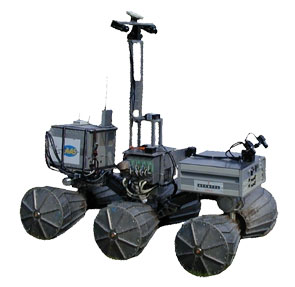
\includegraphics[width=0.9cm]{lama-detour-web-small.jpg}
}


\figw{./figures/lama-components-112002}{\textwidth}

\end{frame}

%----------------------------------------------------------------------
\begin{frame}
\frametitle{Sample modules: Karma  \hfill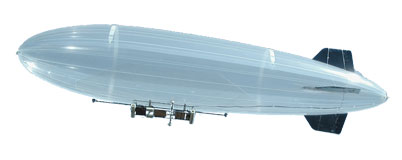
\includegraphics[width=1.7cm]{karma-detour-web-small.jpg}
}

\figw{karma-components.pdf}{\textwidth} 
\end{frame}

%----------------------------------------------------------------------
\begin{frame}
\frametitle{Sample modules: Rackham  \hfill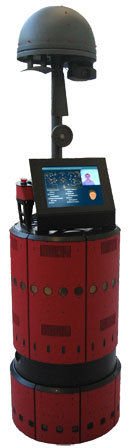
\includegraphics[width=0.25cm]{rackham-detour-web-small.jpg}
}


\figw{rackham-components.png}{8.5cm} 

\end{frame}

%----------------------------------------------------------------------
\begin{frame}
\frametitle{How to communicate with a module?}

\textbf{Requests} (\texttt{msgLib})

\vspace{1em}
\figw{./figures/moduleRqst2}{11cm}

\begin{center} \textbf{$\rightarrow$ control flow} \end{center}
\end{frame}

%----------------------------------------------------------------------
\begin{frame}
\frametitle{How to communicate with a module?}

\textbf{Posters} (\texttt{posterLib})

\vspace{1em}
\figw{./figures/modulePoster}{\textwidth}

\begin{center}  \textbf{$\rightarrow$ data flow}  \end{center}

\texttt{pocolibs} (\url{http://softs.laas.fr/openrobots})

\end{frame}


%----------------------------------------------------------------------
\begin{frame}
\frametitle{Behavior of a module: control request}

%%
%% METTRE LES FLECHES EN PARLANT
%%

\figw{./figures/module-fonctionmt}{6cm}

\end{frame}

%----------------------------------------------------------------------
\begin{frame}
\frametitle{Behavior of a module: execution request}

%%
%% METTRE LES FLECHES EN PARLANT
%%

\figw{./figures/module-fonctionmt2}{6cm}

\end{frame}


%----------------------------------------------------------------------
\begin{frame}
\frametitle{Development cycle of a module}


\figw{figures/cycle}{\textwidth}

7 steps (including 4 ``transparent''):
{\small
\begin{center}
\begin{tabularx}{\linewidth}{ll|X}
\bf 1. & \textbf{describe the module:} edit the \texttt{.gen} file, & \\
 2. \& 3. & generate + build the module (\texttt{make}), & iterate \\ 
\bf 4. & \textbf{write the algorithms} (codels), &  while \\
 5. \& 6. & compile codels +  & needed \\
	& link edition with the module (\texttt{make}), & \\
\bf 7. & \textbf{test the module.} & 
\end{tabularx}
\end{center}}


\end{frame}
%----------------------------------------------------------------------
\begin{frame}
\frametitle{Summary of 1st part}


\begin{tabbing}
\textbf{Module: } \=
 database\\
 \> + processing functions  (set of \textbf{codels})\\
 \> + execution engine
\end{tabbing}

\textbf{Requests:} control and execution 

\textbf{Posters:} data transfers

\textbf{Activity:}  executing process of a request

\end{frame}
%----------------------------------------------------------------------
\section{How to write a module}
\label{edition}
%----------------------------------------------------------------------

\begin{frame}[fragile]
\frametitle{Directories setup}

General configuration:

\begin{itemize}
\item Use \emph{Robotpkg} to install genom and its dependencies.
\item Openrobots tools installed in \verb|$prefix| (\texttt{\$HOME/openrobots}) 
%$

\item Environment variables:
\begin{itemize}
\item PATH \verb|$prefix/bin| %$
\item PKG\_CONFIG\_PATH \verb|$prefix/lib/pkgconfig| %$
\end{itemize}
\end{itemize}

\vspace{1ex}
Directory layout for \texttt{demo}:\\
\vspace{.5ex}
{\small
\begin{tabular}{|l|ll|}
\hline
\texttt{demo/}  & module description  & \texttt{demo.gen} \\
		& data structures   & \texttt{demoStruct.h} \\
\hline
\texttt{demo/server/}  & server & (generated by \GenoM{}) \\
\hline
\texttt{demo/autoconf/} & autotools scripts &\\
\hline
\texttt{demo/codels/}  &  algorithms (codels) & \tt demoXxxCodels.c\\
\hline
\end{tabular}}


\end{frame}

%----------------------------------------------------------------------
\begin{frame}
\frametitle{Components of a module description}

The \texttt{demo.gen} file describes:

\begin{itemize}
\item module (name + identifier)
\item internal database (C structure)
\item requests 
\item posters
\item execution tasks
\end{itemize}

\end{frame}


%----------------------------------------------------------------------
\begin{frame}[containsverbatim]
\frametitle{Edition of the module: XEmacs \texttt{genom} mode}

Configuration file \texttt{.emacs.d/init.el}
\vspace*{.5cm}
{\footnotesize
\begin{lstlisting}
(setq load-path 
  (cons (expand-file-name "~/openrobots/share/genom")  
        load-path))
(setq auto-mode-alist 
  (cons '("\\.gen$" . genom-mode) auto-mode-alist))
(autoload 'genom-mode "genom-mode" "Genom-mode" t)
\end{lstlisting} 
}
%$

(currently broken with modern emacs versions)

\end{frame}

%----------------------------------------------------------------------

\begin{frame}
\frametitle{Emacs Genom mode}

Commands (or menu):

\vspace{1em}
\begin{tabularx}{\linewidth}{|l|X|}
\hline
\tt C-c C-m & \textbf{m}odule creation ({\em 1st command to call})\\
\tt C-c C-i & \textbf{i}mportation de structures \\
\tt C-c C-r & \textbf{r}equest creation \\
\tt C-c C-p & \textbf{p}oster creation\\
\tt C-c C-e & \textbf{e}xecution task creation\\
\hline
\tt C-c C-b & \textbf{b}uffer indentation \\
\tt C-c C-v & \textbf{v}erify fields syntax \\
\tt C-c C-d & \textbf{d}elete unused fields \\
\hline
\tt C-c C-h \ldots & \textbf{h}elp on line\\
\hline
\end{tabularx}


\end{frame}

%----------------------------------------------------------------------
\begin{frame}
\frametitle{A first module example}

How to control the motion of a mobile moving along one axis ?

\vspace{1em}
\figw{figures/mobile}{6cm}


\begin{itemize}
\item {\bf One main service}: "move the mobile to a given position"\\
$\Rightarrow$ {\bf execution request}: \texttt{Goto}
%\vspace{-.8cm}
		\begin{itemize}
		\item input: \texttt{position} to reach
		\end{itemize}
\item {\bf parameters control}: "get or change speed reference"\\
	 $\Rightarrow$ {\bf control request}: 
		\begin{itemize}
		\item \texttt{SetSpeed} with input: new speed reference
		\item \texttt{GetSpeed} with output: current speed reference
		\end{itemize}
\end{itemize}
\end{frame}

%----------------------------------------------------------------------
\begin{frame}[containsverbatim]
\frametitle{Edition of \texttt{demo.gen}: module declaration}

%\vspace*{-0.3cm}
\textbf{\texttt{C-c C-m demo}}
%\vspace*{-0.2cm}
{\tiny
\begin{lstlisting}
/*-------------------------------------------------------
 *               --  Module  DEMO  --
 *
 *  Description:       The only purpose is to do a demo
 *  Creation date:     Sat Jul 15 13:20:11 CEST 2006
 *  Author:            Sara Fleury
 *--------------------------------------------------------

module demo {
     number:          <<number>>;
     version:         "0.1";
     email:           <email>;
     requires:        <package-or-module> ...;
     internal_data:   DEMO_STR;
     uses_cxx:        0;
}; 

/*-------------------------------------------------------
 *               Structures and IDS
 *-------------------------------------------------------*/
#include "demoStruct.h"

typedef struct DEMOCAL_STR {

} DEMOCAL_STR;
\end{lstlisting}
}
\end{frame}

%----------------------------------------------------------------------
\begin{frame}[containsverbatim]
\frametitle{\texttt{demo.gen}: creation of a control request}

{\footnotesize
\begin{lstlisting}
/*--------------------------------------------------
 *             Requests 
 *--------------------------------------------------*/

request SetSpeed {
    doc:                  "<some doc>";
    type:                 control;
    input:                <name>::<sdi-ref>; 
    input_info:           <default-value>::"<doc>" , ...;
    output:               <name>::<sdi-ref>; 
    c_control_func:       demoSetSpeedCntrl;
    fail_msg:             <msg-name> , ...;
    interrupt_activity:   <exec-rqst-name> , ...;
};
\end{lstlisting}
}
\end{frame}

%----------------------------------------------------------------------
\begin{frame}[containsverbatim]
\frametitle{\texttt{demo.gen}: creation of an execution request}

{\footnotesize
\begin{lstlisting}
request Goto {  
    doc:                  "<some doc>";
    type:                 exec;
    exec_task:            <<exec-task-name>>; 
    input:                <name>::<sdi-ref>; 
    input_info:           <default-value>::"<doc>" , ...;
    posters_input:        <struct-name>, ...;
    output:               <name>::<sdi-ref>; 
    c_control_func:       demoGotoCntrl;
    c_exec_func_start:    demoGotoStart; 
    c_exec_func:          demoGotoExec; 
    c_exec_func_end:      demoGotoEnd; 
    c_exec_func_inter:    demoGotoInter; 
    fail_msg:             <msg-name> , ...; 
    interrupt_activity:   Goto, <exec-rqst-name>, ...; 
};
\end{lstlisting}
}
\end{frame}

%----------------------------------------------------------------------
\begin{frame}[containsverbatim]
\frametitle{\texttt{demo.gen}: creation of a poster}
\vspace*{1cm}

{\footnotesize
\begin{lstlisting}
poster Status {
    update:              auto;
    data:                <<name>>::<<sdi-ref>> , ...;
    exec_task:           <<exec-task-name>>; 
};
\end{lstlisting}
}
\end{frame}

%----------------------------------------------------------------------
\begin{frame}[containsverbatim]
\frametitle{\texttt{demo.gen}: creation of an execution task}
\vspace*{1cm}

{\small
\begin{lstlisting}
exec_task MotionTask {
    period:              <number>;
    delay:               <number>;
    priority:            <<number>>;
    stack_size:          <<number>>;
    c_init_func:         demoMotionTaskInit;
    c_func:              demoMotionTaskPerm;
    c_end_func:          demoMotionTaskEnd;
    fail_msg:            <msg-name> , ...;
};
\end{lstlisting}}

\end{frame}


%----------------------------------------------------------------------
\begin{frame}[containsverbatim]
\frametitle{Description of the module \texttt{demo.gen}}

{\scriptsize
\begin{lstlisting}
/* ---- Module declaration ---- */
module demo {
     number:                9000;
     internal_data:         DEMO_STR;
     version:         "0.1";
     email:           sara@laas.fr;
     internal_data:   DEMO_STR;
     uses_cxx:        0;
};

/* ---- Structure definitions ---- */
#include "demoStruct.h"
#include "demoConst.h"

/* ---- Database of the module ---- */
typedef struct DEMO_STR {
     DEMO_STATE_STR state;         /* Current state */
     DEMO_SPEED     speedRef;      /* Speed reference */
     double         posRef;        /* Position reference */
     double         monitor;       /* Positions monitors */
}DEMO_STR;
\end{lstlisting}
}
\end{frame}

%----------------------------------------------------------------------
\begin{frame}[containsverbatim]
\frametitle{Description of the module \texttt{demo.gen} (cont.)}


{\scriptsize
\begin{lstlisting}
/* ---- declaration of the services: the requests ---- */

/* Control requests */
request SetSpeed {
    doc:                 "To change speed";
    type:                control;
    input:               speed::speedRef;
    input_info:          DEMO_DEFAULT_SPEED::"DEMO_SLOW or DEMO_FAST";
    c_control_func:      controlSpeed;
    fail_msg:            INVALID_SPEED;
};

request GetSpeed {
    doc:                 "To get current speed value";
    type:                control;
    output:              speed::speedRef;
};
\end{lstlisting}
}
\end{frame}

%----------------------------------------------------------------------
\begin{frame}[containsverbatim]
\frametitle{Description of the module \texttt{demo.gen} (cont. 2)}

{\scriptsize
\begin{lstlisting}
/* Execution requests */
request Goto {
    doc:                    "Goto the given position";
    type:                   exec;
    input:                  goal::posRef;
    input_info:             0::"position in m";
    c_control_func:         demoGotoCntrl;
    fail_msg:               TOO_FAR_AWAY;
    c_exec_func_start:      demoGotoStart;
    c_exec_func:            demoGotoExec;
    c_exec_func_end:        demoGotoEnd;
    c_exec_func_inter:      demoGotoEnd;
    interrupt_activity:     Goto;
    exec_task:              MotionTask;
};
\end{lstlisting}
}

\end{frame}
%----------------------------------------------------------------------
\begin{frame}[containsverbatim]
\frametitle{\texttt{demo}: structures and constants}

{\scriptsize
\begin{lstlisting}
#ifndef DEMO_STRUCT_H
#define DEMO_STRUCT_H

typedef struct DEMO_STATE_STR {
  double position;  /* currente position (m) */
  double speed;     /* current speed (m/s) */
} DEMO_STATE_STR;

typedef enum DEMO_SPEED {
  DEMO_SLOW, 
  DEMO_FAST
} DEMO_SPEED;
#endif
\end{lstlisting}
}
\vspace{1em}

{\scriptsize
\begin{lstlisting}
#ifndef DEMO_CONST_H
#define DEMO_CONST_H
#define DEMO_MACHINE_LENGTH    20.0       /* m */
#define DEMO_DEFAULT_SPEED     DEMO_FAST  /* DEMO_SLOW */
#endif
\end{lstlisting}
}

\end{frame}

%----------------------------------------------------------------------
\begin{frame}
\frametitle{Summary of 2nd part}


3 files to describe a module:
	\begin{itemize}
	\item description file \texttt{demo.gen}
	\item structures \texttt{demoStruct.h}
	\item constants \texttt{demoConst.h}
	\end{itemize}

5 parts in the  \textbf{.gen} file:
	\begin{itemize}
	\item module (name + identifier)
	\item database (data structures)
	\item requests
	\item posters
	\item execution tasks
	\end{itemize}

\end{frame}
%----------------------------------------------------------------------
\section{How to generate a module}
%----------------------------------------------------------------------
\begin{frame}[containsverbatim]
\frametitle{First generation of the module: \texttt{genom demo.gen}}

%\vspace{0.1cm}

%Commande: \texttt{genom -i demo.gen}

{\tiny
\begin{lstlisting}
blues% genom demo.gen
genom demo.gen: info: array MonitorInput added in SDI for request Monitor
genom demo.gen: info: array MonitorOutput added in SDI for request Monitor
perl -w ./demo.pl

Updating top directory
  creating autogen

Updating codels
  demoMotionTaskCodels.c changed, skipping
  demoCntrlTaskCodels.c changed, skipping
  Makefile.in changed, skipping

Updating autoconf
  creating genom.mk
...
Updating server
  creating Makefile.in
...
Creating build environment ...
  * Running aclocal
  * Running autoconf

If you already have a build of this module, do not forget to
reconfigure (for instance by running ./config.status --recheck)

Done.
\end{lstlisting}
}
\end{frame}
%----------------------------------------------------------------------
\begin{frame}[containsverbatim]
\frametitle{GenoM outputs}

Production of several files and directories:
%\vspace{-1cm}
\begin{itemize}
\item \texttt{Makefile.in}, \texttt{configure}...
\item \texttt{server/}, \texttt{autoconf} and \texttt{codels/}
\end{itemize}

{\footnotesize
\begin{lstlisting}
autogen*            configure.ac.user   local.mk.in 
Makefile.in         demo.gen            server/
acinclude.user.m4   codels/             demoConst.h         
autoconf/           configure*          demoStruct.h        
\end{lstlisting}
}

\end{frame}
%----------------------------------------------------------------------
\begin{frame}
\frametitle{GenoM outputs: the server}


In \texttt{demo/server/} files used by genom and clients of the module, related to:
\begin{itemize}
\item server: 
	\texttt{demoCntrlTask, demoMotionTask, \ldots}
\item libraries to send requests and receive replies
	\texttt{demoMsgLib}
\item libraries to access posters:
	\texttt{demoPosterLib}
\item Test program:
	\texttt{demoTest.c}
\end{itemize}
\end{frame}
%----------------------------------------------------------------------
\begin{frame}
\frametitle{GenoM outputs: codels}

In \texttt{demo/codels/}
files that will contain the algorithms.

1 codels file per task:

\begin{itemize}
\item Control codels:
 \texttt{democCntrlTaskCodels.c}
\item Execution codels:
 \texttt{demoMotionTaskCodels.c}
\item Autoconf infrastructure:
\texttt{Makefile.in} \texttt{autoconf/} \texttt{configure}
\end{itemize}

\end{frame}

%----------------------------------------------------------------------
\begin{frame}[containsverbatim]
\frametitle{Configuring the module}

Create a build directory:

{\scriptsize
\begin{lstlisting}
blues% mkdir build
blues% cd build
\end{lstlisting}}

Call configure, telling where to install the module:

{\scriptsize
\begin{lstlisting}
blues% ../configure --prefix=${HOME}/openrobots
checking build system type... i686-pc-linux-gnu
checking host system type... i686-pc-linux-gnu
checking for gcc... gcc
checking for C compiler default output file name... a.out
...
config.status: creating codels/Makefile
config.status: creating server/Makefile
config.status: creating demo.pc
config.status: creating local.mk
\end{lstlisting}}
\end{frame}
%----------------------------------------------------------------------
\begin{frame}[containsverbatim]
\frametitle{Building the module}

Call: \texttt{make}

\begin{itemize}
\item re-generates the module if needed
\item builds everything
\end{itemize}

{\tiny
\begin{lstlisting}
blues% make
make all-posix
make[1]: Entering directory `/home/foo/openrobots/modules/demo/build'
make[2]: Entering directory `/home/foo/openrobots/modules/demo/build/server'
mkdir -p posix-build
/home/foor/openrobots/bin/mkdep -c"gcc" -oposix-build/dependencies -dposix-build 
-t.lo -DUNIX    -I. -I../.. -I../../server -I/home/foo/openrobots/include   
../../server/demoCntrlTask.c ../../server/demoModuleInit
...
creating posix-build/demo
make[2]: Leaving directory `/home/foo/openrobots/modules/demo/build/codels'
make[1]: Leaving directory `/home/foo/openrobots/modules/demo/build'

\end{lstlisting}}

\end{frame}

%----------------------------------------------------------------------
\begin{frame}[containsverbatim]
\frametitle{Installation}
The module needs to be installed to be useful.

\vspace{1em}
{\small
\begin{lstlisting}
blues% make install
\end{lstlisting}}

\vspace{1em}
It is installed as specify with the \texttt{--prefix} option of \texttt{configure}.

According to the destination you have chosen, you may need \texttt{root} priviledges.
\end{frame}
%----------------------------------------------------------------------
\begin{frame}
\frametitle{Summary of 3rd part}


\begin{enumerate}
\item Edit the module: {\bf demo.gen}

\item Only the first time: generate {\bf genom} \\
  and configure {\bf configure}

\item Compile and generate: {\bf make}

\item Install: {\bf make install}

\end{enumerate}

\end{frame}

%----------------------------------------------------------------------
\section{How to run a module}
%----------------------------------------------------------------------
\begin{frame}[containsverbatim]
\frametitle{UNIX session: execution}


1. Start the communication server:

\begin{lstlisting}
blues% h2 init
\end{lstlisting}

2. Start the module:

\begin{lstlisting}
blues% demo -b
\end{lstlisting}

\texttt{-b} option allows to wait until the module has effectively
started.

3. Start the client(s):

\begin{lstlisting}
blues% demoTest 1
\end{lstlisting}

\end{frame}


%----------------------------------------------------------------------
\begin{frame}[containsverbatim]
\frametitle{The test program \texttt{demoTest} }

{\scriptsize
\begin{lstlisting}
blues% demoTest 1 
pocolibs execution environment version 2.8
Copyright (c) 1999-2010 CNRS-LAAS
client init ...ok.   Poster init ...ok.
---------------------------------------------------------------------
  0: SetSpeed              2: Stop                4: GotoPosition (E)
  1: GetSpeed              3: MoveDistance (E)    5: Monitor (nE)

55: posters  66: abort  77: replies(0)  88: state  99: QUIT  -99: END
---------------------------------------------------------------------
demo1 (88)> 
\end{lstlisting}
}

\end{frame}

%----------------------------------------------------------------------
\begin{frame}[containsverbatim]
\frametitle{The test program \texttt{demoTest} (cont) }

{\scriptsize
\begin{lstlisting}
demo1 (88)> 3

Get current distRef using poster Mobileref (y/n) ? (n) 

-- Enter double distRef:  (0.000000) 1.0
Wait final reply (y/n/a) ? : y

Activity 0 started
start engine
stop engine
Final reply: OK

---------------------------------------------------------------------
  0: SetSpeed              2: Stop                4: GotoPosition (E)
  1: GetSpeed              3: MoveDistance (E)    5: Monitor (nE)

55: posters  66: abort  77: replies(0)  88: state  99: QUIT  -99: END
---------------------------------------------------------------------
demo1 (3)> 
\end{lstlisting}}

\end{frame}

%----------------------------------------------------------------------
\begin{frame}[containsverbatim]
\frametitle{UNIX  session: end}

\begin{enumerate}
\item Kill the module:

\begin{lstlisting}
blues% killmodule demo
\end{lstlisting}

or with the command \texttt{-99} in the \texttt{demoTest} menu.

{\bf (then one can restart the module)}


\item end the session:

\begin{lstlisting}
blues% h2 end
\end{lstlisting}

\end{enumerate}
\end{frame}

%----------------------------------------------------------------------
\begin{frame}
\frametitle{Summary of 4th part}

\begin{enumerate}
\item Edit the module: {\bf demo.gen}

\item Only the first time: generate ({\bf genom}) and configure ({\bf configure})

\item (Re) generate and compile: {\bf make}

\item Install: {\bf make install}

\item Execute: {\bf h2 init, demo -b, demoTest 1, ... h2 end}

\end{enumerate}

\end{frame}

%----------------------------------------------------------------------
\section{How to integrate algorithms}
%----------------------------------------------------------------------
\begin{frame}
\frametitle{Codels}

\bi

\item All the codels are in the directory: {\tt codels/}

\item In this directory we have one codels file per task.

\item Thus for the \texttt{demo} we have:

\begin{itemize}
\item {\tt demoCntrlTaskCodels.c} for the control codels ({\tt c\_control\_func})

\item {\tt demoMotionTaskCodels.c} for the execution codels ({\tt
c\_exec\_func}, \ldots)

\end{itemize}
\end{itemize}
\end{frame}

%----------------------------------------------------------------------
\begin{frame}[containsverbatim]
\frametitle{Control codels}

{\scriptsize
\begin{lstlisting}
STATUS demoSetSpeedCntrl(DEMO_SPEED *speed, int *report)
{
   /* Refuse *speed if the value is erroneous */
   if (*speed != DEMO_SLOW && *speed != DEMO_FAST) {
        *report = S_demo_INVALID_PARAMETER; return ERROR;
   }
   /* Parameter is valid: it will be recorded into the fIDS */
   return OK;
}

STATUS demoGotoCntrl(double *posRef, int *report)
{
   /* Refuse *posRef if the value is erroneous */
   if (fabs(*posRef) > DEMO_MCHINE_LENGTH/2.0) {
        *report = S_demo_INVALID_PARAMETER; return ERROR;
   }
   /* Parameter is valid: it will be recorded into the fIDS 
      and Goto request will start */
   return OK;
}
\end{lstlisting}}

\end{frame}


%----------------------------------------------------------------------
\begin{frame}[containsverbatim]
\frametitle{Execution codels}

{\scriptsize
\begin{lstlisting}
ACTIVITY_EVENT demoGotoStart(double *posRef, int *report)
{
   printf("Start engine\n");
   return EXEC;
}

ACTIVITY_EVENT demoGotoExec(double *posRef, int *report)
{
   double dist = *posRef - SDI_f->state.position;
   switch(SDI_f->speedRef) {
       case DEMO_SLOW:
	    if (fabs(dist) < 0.1) return END;
	    SDI_f->state.position += sign(dist) * 0.1;
	    return EXEC;
       case DEMO_FAST:
	    if (fabs(dist) < 1) return END;
	    SDI_f->state.position += sign(dist) * 1;
	    return EXEC;
   }
}
\end{lstlisting}}
\end{frame}

%----------------------------------------------------------------------
\begin{frame}[containsverbatim]
\frametitle{Execution codels (cont)}

{\scriptsize
\begin{lstlisting}
ACTIVITY_EVENT demoGotoEnd(double *posRef, int *report)
{
   SDI_f->state.position = *posRef;
   printf("Stop engin\n");
   return ETHER;
}
\end{lstlisting}}
\end{frame}
%----------------------------------------------------------------------
\begin{frame}[containsverbatim]
\frametitle{Specific codels}

\bi
\item Initialisation codel {\tt c\_init\_func} 
\item Terminaison codel  {\tt c\_end\_func} 
\item Permanent activity codel: {\tt c\_func}
\ei

$\rightarrow$ one per execution task  \\

{\scriptsize
\begin{lstlisting}
#include "demoConst.h"

STATUS demoComputeInit(int *report)
{
  SDI_F->state.position = 0.0;
  SDI_F->state.speed = 0.0;
  SDI_F->posRef = 0.0
  SDI_F->speedRef = DEMO_SLOW
  return OK;
}
\end{lstlisting}}
\end{frame}

%----------------------------------------------------------------------
\begin{frame}
\frametitle{Summary of 5th part}

\begin{enumerate}
\item Edit the module: {\bf demo.gen}

\item Only the first time: generate ({\bf genom}) and configure ({\bf configure})

\item (Re) generate and compile: {\bf make}

\item Install: {\bf make install}

\item Execute: {\bf h2 init, demo -b, demoTest 1, ... h2 end}

\item Fill-in the codels (and goto {\bf 3})

\end{enumerate}

\end{frame}

%----------------------------------------------------------------------
\section{Codels and activities}
%----------------------------------------------------------------------
\begin{frame}
\frametitle{Activities and codels}

\bi
\item generally:
1 activity $\rightarrow$ a sequence of codels:

{\tt start}\\
{\tt exec}\\
{\tt exec}\\
{\tt \ldots}\\
{\tt exec}\\
{\tt end}
\ei


\bi
\item Codels are not interruptible
\item Activity are interruptible on transitions between 2 codels.
\item On Interruption $\Rightarrow$ execution of the codel {\tt inter}
\ei 

\end{frame}
%----------------------------------------------------------------------
\begin{frame}[containsverbatim]
\frametitle{Execution requests and codels}

One example:

{\footnotesize
\begin{lstlisting}
/* Translation on a given distance */
request Goto {
   type:                exec;               
   input:               distance::distRef;  
   c_control_func:      demoGotoCntrl;
   fail_msg:            TOO_FAR_AWAY;       
   c_exec_func_start:   demoGotoStart;     
   c_exec_func:         demoGotoExec;   
   c_exec_func_end:     demoGotoEnd;      
   c_exec_func_inter:   demoGotoInter;      
   interrupt_activity:  Goto;       
   exec_task:           MotionTask;         
};
\end{lstlisting}
}
\end{frame}
%----------------------------------------------------------------------
\begin{frame}[containsverbatim]
\frametitle{Activities decomposition in codels}

\figw{figures/grapheExec}{5cm}

\vspace{1em}
{\footnotesize
\begin{tabularx}{\linewidth}{|l|l|X|}
\hline
�tat 	 	& codel (if exists)	&  \\
\hline
\tt START  & \tt c\_exec\_func\_start  	& starting	\\
\tt EXEC   & \tt c\_exec\_func  	& main \\
\tt END    &\tt c\_exec\_func\_end 	& terminating \\
\tt FAIL   & \tt c\_exec\_func\_fail 	& terminating (pb) \\
\hline
\tt INTER  & \tt c\_exec\_func\_inter  	& terminating (on interruption) \\
\hline
\tt SLEEP  & 				& wait event \\
\tt ETHER    &	& \em activity over   \\
\tt ZOMBIE   &	& \em activity suspended  \\
\hline
\end{tabularx}}

\end{frame}


%----------------------------------------------------------------------
\begin{frame}[containsverbatim]
\frametitle{Periodical task}

$\rightarrow$ Periodical task \\

{\footnotesize
\begin{lstlisting}
exec_task Compute {
    period:                10;     /* 100ms */
    priority:              20;     /* a hight priority */
    stack_size:            10000;
};
\end{lstlisting}}

\bi
\item usely 1 tic = 10ms on Unix/Linux
\item priority: [0..255] (0: higher priority): \\
  used only on real-time OS
\item stack\_size: used only on real-time OS
\ei

\end{frame}

%----------------------------------------------------------------------
\begin{frame}[containsverbatim]
\frametitle{The posters: automatics or manual}

Exporting results

\bi
\item Automatical update every time its execution task wakes~up

{\scriptsize
\begin{lstlisting}
poster Status {
    update:              auto;
    data:                state::state;
    exec_task:           MotionTask;
};
\end{lstlisting}
}

\item Manual update only when necessary

{\scriptsize
\begin{lstlisting}
poster Status {
    update:              user;
    type:                SPEED_REF;
    exec_task:           MotionTask;
};
\end{lstlisting}
}
\ei 
\end{frame}
%----------------------------------------------------------------------
\begin{frame}[containsverbatim]
\frametitle{Posters:  manual update}
Update from a codel: \\

{\footnotesize
\begin{lstlisting}
ACTIVITY_EVENT demoGotoStart(double *posRef, int *report)
{
   printf("Start engin\n");
   if (demoStatusSPEED_REFPosterWrite 
                         (DEMO_STATUS_POSTER_ID,
                          SDI_F->speedRef) != OK) {
    *report = S_demo_CANNOT_WRITE_POSTER;
    return ETHER;
  }
   return EXEC;
}
\end{lstlisting}
}

\end{frame}
%----------------------------------------------------------------------
\begin{frame}
\frametitle{Summary of 6th part}

\begin{enumerate}
\item Edit the module: {\bf demo.gen}

\item Only the first time: generate ({\bf genom}) and configure ({\bf configure})

\item (Re) generate and compile: {\bf make}

\item Install: {\bf make install}

\item Execute: {\bf h2 init, demo -b, demoTest 1, ... h2 end}

\item Fill-in the codels (and goto {\bf 3})

\end{enumerate}

\end{frame}
%----------------------------------------------------------------------
\section{How to use a module}
%----------------------------------------------------------------------
\begin{frame}[containsverbatim]
\frametitle{Using module structures from another module}

Import structures: 

{\scriptsize
\begin{lstlisting}
module pilo {
     number:          9000;
     version:         "0.1";
     requires:        demo;
     internal_data:   PILO_STR;
}; 

import from demo {
#include "demoStruct.h"
};
#include "piloStruct.h"

typedef struct PILO_STR {
     PILO_GOTO_STR goto;
     DEMO_POS_REF  posRef;
} PILO_STR;
\end{lstlisting}
}

Based on \texttt{pkgconfig}.
\end{frame}

%----------------------------------------------------------------------
\begin{frame}[containsverbatim]
\frametitle{Read a poster from another module}

{\scriptsize
\begin{lstlisting}
request Track {
   type:   exec;
   ...
   posters_input:    LOCO_SPEED_REF;
   ...
};

\end{lstlisting}
}

Library: {\tt demoPosterReadLib}

{\tiny
\begin{lstlisting}
  POSTER_ID trackPosterId=-1;
  DEMO_REF ref;

  /* look for the poster */
  if (posterFind(track->posterName, &trackPosterId) == ERROR) {
    *report = S_demo_CANNOT_FIND_POSTER;
    return ETHER;
  }
  /* try to read the data for the first time */
  if (demoDEMO_REFPosterRead(trackPosterId, &ref) == ERROR) {
    *report = S_demo_CANNOT_READ_POSTER;
    return ETHER;
  }
...

\end{lstlisting}
}

\end{frame}

%----------------------------------------------------------------------
\begin{frame}[containsverbatim]
\frametitle{Control of a module with tclserv: principle}


\begin{itemize}
\item {\tt tclServ} allows to control a set of modules from a unique interface

\item Full interactive programming language (Tcl)

\item ASCII data transfers (non sensitive to data representation like little endian / big endian / alignment).

\item Graphical libraries {\tt Tk}
\end{itemize}

\url{http://www.openrobots.org/wiki/eltclsh}

\end{frame}
%----------------------------------------------------------------------
\begin{frame}
\frametitle{Module control with tclserv: usage}

\begin{enumerate}
\item Generate the module with option {\tt -t}

\item Start the server {\tt tclserv}.

\item Start one (or several) tcl-shells:\\
{\tt eltclsh -package genom}


\item Start session (see example).

\end{enumerate}

\end{frame}
%----------------------------------------------------------------------
\begin{frame}
\frametitle{Module control with tclserv: options and commands}
{\center
{\small
\begin{tabularx}{\linewidth}{|l|X|}
\hline
option		& function \\
\hline
\tt -ack & non blocking request sending \\

\tt -raw & the result is presented as a raw list of data
           (not a nice display)  \\
\hline
\end{tabularx}

\vfill
\begin{tabularx}{\linewidth}{|l|X|}
\hline
command		& function \\
\hline
\tt replyof \$rqstId & get answer {\em blocking mode}. 
Generaly used with option {\tt -raw}. \\
\tt cs::term \$rqstId 0 & get answer {\em  non blocking mode}. \\
\tt abort \$rqstId	& abort the request \\
\tt kill $<$module$>$	& abort the module $<$module$>$ \\
\texttt{die} & terminate tclserv and eltclsh itself\\
\hline
\end{tabularx}}
}
\end{frame}

%----------------------------------------------------------------------
\begin{frame}[containsverbatim]
\frametitle{Module control with tclserv: examples}

{\footnotesize
\begin{lstlisting}
eltclsh > connect localhost
connecting to localhost:9472
connected to localhost
eltclsh> lm demo
(re)starting tclServ cs daemon on port 9472
demo loaded on localhost from ~/openrobots/share/modules
eltclsh > ::demo::MoveDistance 
distance in m [0]> 0.5
status = OK
eltclsh > 

\end{lstlisting}
}
\end{frame}
%----------------------------------------------------------------------
\begin{frame}[containsverbatim]
\frametitle{Module control with tclserv: examples (cont.)}

{\small
\begin{lstlisting}
    set demFused [dem::FuseDem -ack]
    set classifDone [lclassif::Classif -ack]
    replyof $demFused

\end{lstlisting} %$
}
\end{frame}

%----------------------------------------------------------------------
\begin{frame}
\frametitle{Module control with tclserv: Tk and Gdhe}


Modular and extensible 3D graphical interface with the \texttt{Tk} GUI toolkit:
\begin{itemize}
\item Gdhe \url{http://gdhe.openrobots.org/}
\end{itemize}

3D model of many robots (rackham, jido, dala, mana,...). 

\figw{./figures/gdhe-robots.png}{10cm}

\end{frame}
%----------------------------------------------------------------------
\begin{frame}
\frametitle{Module control with OpenPRS: principle}

\url{http://openprs.openrobots.org/}

\begin{itemize}
\item Supervision
\item Generate the module with option {\tt -o}
\end{itemize}

OPs producted for each request:
{\center
{\small
\begin{tabularx}{\linewidth}{|l|X|}
\hline
nom		& function \\
\hline
\tt DEMO-MOTION & send the request  {\em and} receive the {\em
                    finale reply in blocking mode} \\

\tt DEMO-MOTION-REPORT & idem with the report  \\

\tt DEMO-MOTION-ASYNC & send the request in non blocking mode. \\

\hline
\end{tabularx}}
}

The answer is a string in the data base:
\\
{\tt (FR DEMO DEMO\_MOTION \$RQST-ID \$REPORT \$DATA)}.

\end{frame}

%----------------------------------------------------------------------
\begin{frame}[containsverbatim]
\frametitle{Module control with OpenPRS: {\tt transgen}}

\begin{itemize}
\item Automatic production of OpenPRS relocatable.
\item Similar to GenoM:

\begin{itemize}
\item  Description  file {\tt manip.tg}:
\end{itemize}


{\small
\begin{lstlisting}
/* --- Declaration of a supervisor --- */
supervisor manip {
  module: xr4000;
  module: sick;
  module: m2d;
  module: segloc;
}
\end{lstlisting}
}
\end{itemize}
\end{frame}

%----------------------------------------------------------------------
\begin{frame}[containsverbatim]
\frametitle{Module control with OpenPRS: {\tt transgen} (continued)}

\begin{itemize}
\item Call: {\tt tranGen manip.tg}
\item Compile in {\tt server/}.
\item Start OpenPRS: 
\end{itemize}

{\footnotesize
\begin{lstlisting}
blues% server/i386-linux/manip-xOpenPRS -n manip-cabby \
 -x server/data/manip-data.inc -x data/my-data.inc &
\end{lstlisting}
}

\end{frame}

%----------------------------------------------------------------------
\begin{frame}[containsverbatim]
\frametitle{Module control with OpenPRS: Example of procedure}

An OP that automatically starts
the continuous 
localization request  ({\tt SEGLOC-LOCLOOP-ASYNC}) when the
robot losts itself:

{\scriptsize
\begin{lstlisting}
;;;;;;;;;;;;;;;;;;;;;;;;;
;;; |Localize|
;;;;;;;;;;;;;;;;;;;;;;;;;
(defop |Localize|
    :invocation (! (EXECUTE LOC-LOOP))
    :context (& (UNCERTAINTY-LEVEL-1 $X1 $Y1 $T1) 
                (ALARM-LEVEL-1 $L1))
    :body ((IF (! (EXECUTE LOC-LOCAL))
              (! (SPEAK "ok"))
              (! (SEGLOC-LOCLOOP-ASYNC $RQST-ID1))
              (! (CURRENT-MISSION-COMPLETED))
            ELSE
              (! (SPEAK "Bad localization. Try again"))
              (! (FAILED))
           )
          )
)

\end{lstlisting}
}
%$
\end{frame}

%----------------------------------------------------------------------
\section{Conclusions}
%----------------------------------------------------------------------
\begin{frame}
\frametitle{Summary}

\begin{enumerate}
\item Edit the module: {\bf demo.gen}

\item First time only: generate ({\bf genom}) and configure ({\bf configure})

\item (Re) generate and compile: {\bf make}

\item Install: {\bf make install}

\item Execute: {\bf h2 init, demo -b, demoTest 1, ... h2 end}

\item Control with: {\bf tclserv} and {\bf Tcl/Tk} {\tt (eltclsh, elwish,
gdhe)}	or {\bf OpenPRS}

\end{enumerate}

\end{frame}

%----------------------------------------------------------------------
\begin{frame}
\frametitle{Online documents}

\begin{itemize}
\item Official page:
\url{http://genom.openrobots.org/}

\item Robotpkg:
\url{http://robotpkg.openrobots.org/}

\item Mailling-list: \url{openrobots@laas.fr} \url{https://sympa.laas.fr/sympa/info/openrobots}

\item (Intranet) Wiki: 
\url{http:/intranet.laas.fr/robots/wiki}
\end{itemize}
\end{frame}

\end{document}

% LocalWords:  pdfsubject pdftitle pdfkeywords matthieu doc Fleury Herrb Codels
% LocalWords:  adam jpg bis lapa lama jidowanki rackham dala neobotix cont gen
% LocalWords:  genom pdf png msgLib moduleRqst posterLib modulePoster pocolibs
% LocalWords:  softs laas fr openrobots fonctionmt codels usr PKG ONFIG ATH cd
% LocalWords:  demoStruct autoconf autotools demoXxxCodels setq alist autoload
% LocalWords:  mkdir RQST
